\documentclass[a4paper,11pt, twoside]{article}
\usepackage{graphicx}
\usepackage{float}
\usepackage{geometry}
\geometry{left=2.0cm, right=2.0cm, top=2.5cm, bottom=3.5 cm}
\usepackage{lettrine}
\usepackage{enumitem}
\usepackage{changepage}
\usepackage{pdflscape}


%\usepackage[square, authoryear]{natbib}
%\bibliographystyle{dinat} 
  
\usepackage[
backend=bibtex, 
style=alphabetic, 
citestyle=authoryear,
sorting=ynt
]{biblatex}


%\addbibresource{assgn1.bib}

\usepackage{fontspec}


\setmainfont{libertinusserif-regular}[
Path= /Library/Fonts/libertinus-6.4/,
UprightFont= libertinusserif-regular.otf ,
BoldFont= libertinusserif-bold.otf,
ItalicFont = libertinusserif-italic.otf
]

\setsansfont{SF-Pro-Display-Regular}[
Path= /Library/Fonts/ ,
UprightFont= SF-Pro-Display-Regular.otf ,
BoldFont= SF-Pro-Display-Bold.otf ,
ItalicFont = SF-Pro-Display-RegularItalic.otf ,
]
%%%%%%%%%%%% Font Libertine %%%%%%%%%%%%%%%


\usepackage[toc, title]{appendix}

\usepackage{hyperref}

%\usepackage[T1]{fontenc}
%\usepackage{mathptmx}



\usepackage{fancyhdr}
\pagestyle{fancy}
\fancyhf{}

\setlength\headheight{35.65pt}

\lhead{
\includegraphics[height=1.1cm]{nus-logo.png}}
\rfoot{\thepage}


\title{  \textbf{\texttt{TIC2002}} \textsf{\\ \vspace{0.3cm} \huge{INTRODUCTION TO SOFTWARE ENGINEERING
}} \\ \vspace{0.2cm} \Large{\texttt{Semester 1 - AY19/20}} \\ \vspace{0.8cm} \LARGE{Duke Project Report}}
\date{\small\today}

%%%
\usepackage{titlesec}

\newcommand{\chapfnt}{\fontsize{16}{19}}
\newcommand{\secfnt}{\fontsize{14}{16}}
\newcommand{\ssecfnt}{\fontsize{12}{14}}

\titleformat{\chapter}[display]
{\normalfont\chapfnt\bfseries}{\chaptertitlename\ \thechapter}{20pt}{\chapfnt}

\titleformat{\section}
{\normalfont\secfnt\bfseries}{\thesection}{1em}{}

\titleformat{\subsection}
{\normalfont\ssecfnt\bfseries}{\thesubsection}{1em}{}

\titlespacing*{\chapter} {0pt}{50pt}{40pt}
\titlespacing*{\section} {0pt}{0.7ex plus 1ex minus .2ex}{0.3ex plus .2ex}
\titlespacing*{\subsection} {0pt}{3.25ex plus 1ex minus .2ex}{1.5ex plus .2ex}
%%%

\usepackage{multicol}
\setlength\columnsep{11pt}
\hyphenpenalty= 800


\setlength{\parindent}{5cm}

\begin{document}

\maketitle

\begin{table*} [htbp]
\centering
\begin{tabular}{lcr}
\Large{ }}  \\
\hline \\
NAME &		  &Li Shihao \\
MATRIX NO. &		  &A0165362E \\
GITHUB USERNAME &	  	&\href{https://github.com/asmaww/duke}{asmaww} \\
EMAIL &		  &\href{mailto:e0166067@u.nus.edu}{e0166067@u.nus.edu} \\
\end{tabular}
\end{table}
%\tableofcontents


\clearpage


\section* {User Stories} 


\begin{enumerate}[label=\textbf{\arabic*}.]
\item Duke task checklist supports multiple users to use the application; 
\item As users who prefer faster entries, it would be a great fit for this kind of audience to be able to quickly note down and manipulate tasks using various commands, which are triggered by a few key strokes. It's faster than clicking buttons by mouse in GUI;
\item When the next time users start the program, Duke should still remember the tasks that users had left from last time; 
\item There are different types of task that fit in different use cases; 
\item There are commands that mark task status such as completion and provide views of list of tasks; 
\item System should be fast, reliable and provide message to guide correct user behaviour. 
\end{enumerate}


\section* {Non-functional requirements} 
\begin{enumerate}[label=\textbf{\arabic*}.]
\item Message from the system should be fun and intimate;  
\item The system should be smart to guide the users with meaningful alert of what to do rather than just exit;
\item Minimum visual elements/clusters which create distraction for users want to be fast. The aesthetic aims for simplicity and tidiness.  
\end{enumerate}


\section* {Level-1 The output Duke shows when launching the program} 
\begin{figure}[H]
\centering
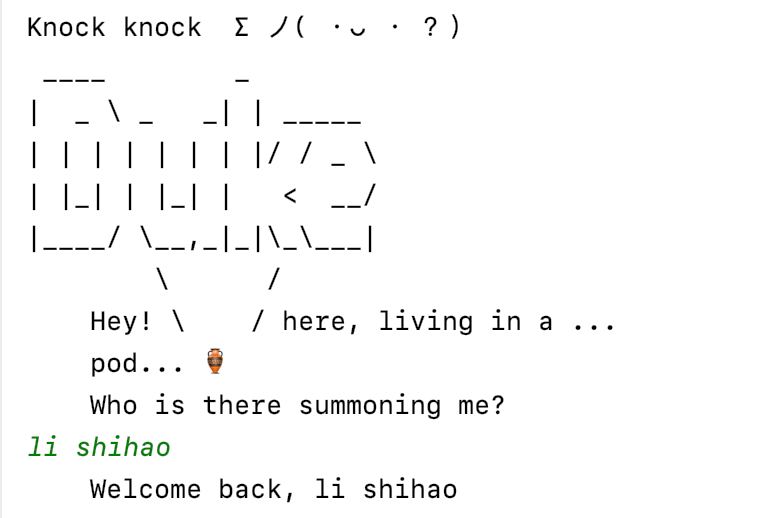
\includegraphics[height= 5.8cm]{startold.png}
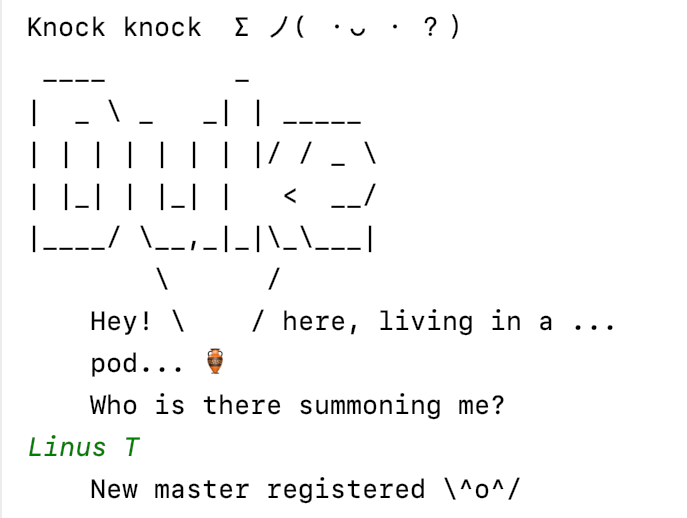
\includegraphics[height= 5.8cm]{startnew.png}
\caption{Screenshot - Start Greeting Page Existing/New User} 
\label{start}
\end{figure} 


\section* {Level-4 Describe the commands for adding different types of tasks} 
\begin{figure}[H]
\left
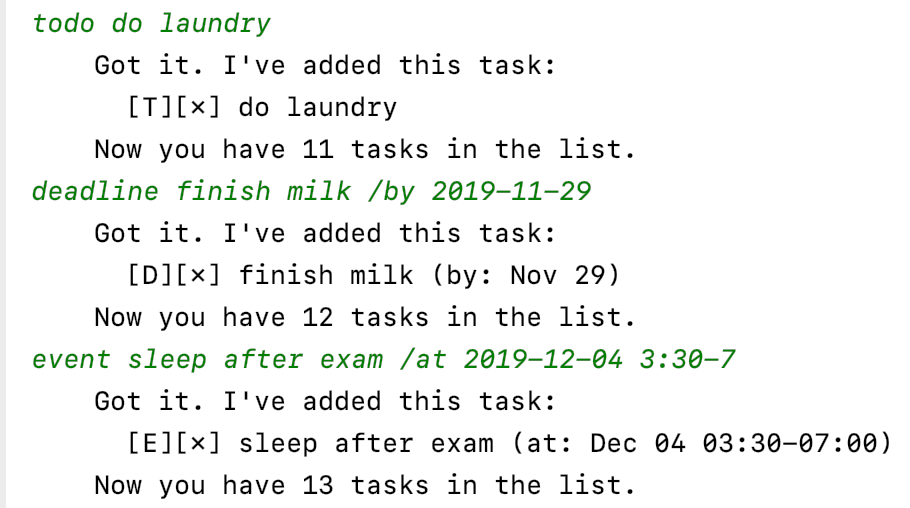
\includegraphics[height= 6 cm]{task.png}

\caption{Screenshot - \texttt{todo, deadline, event}} 
\label{startold}
\end{figure} 

\section* {Level-2  Describe the commands for listing tasks} 

\begin{figure}[h]
\left
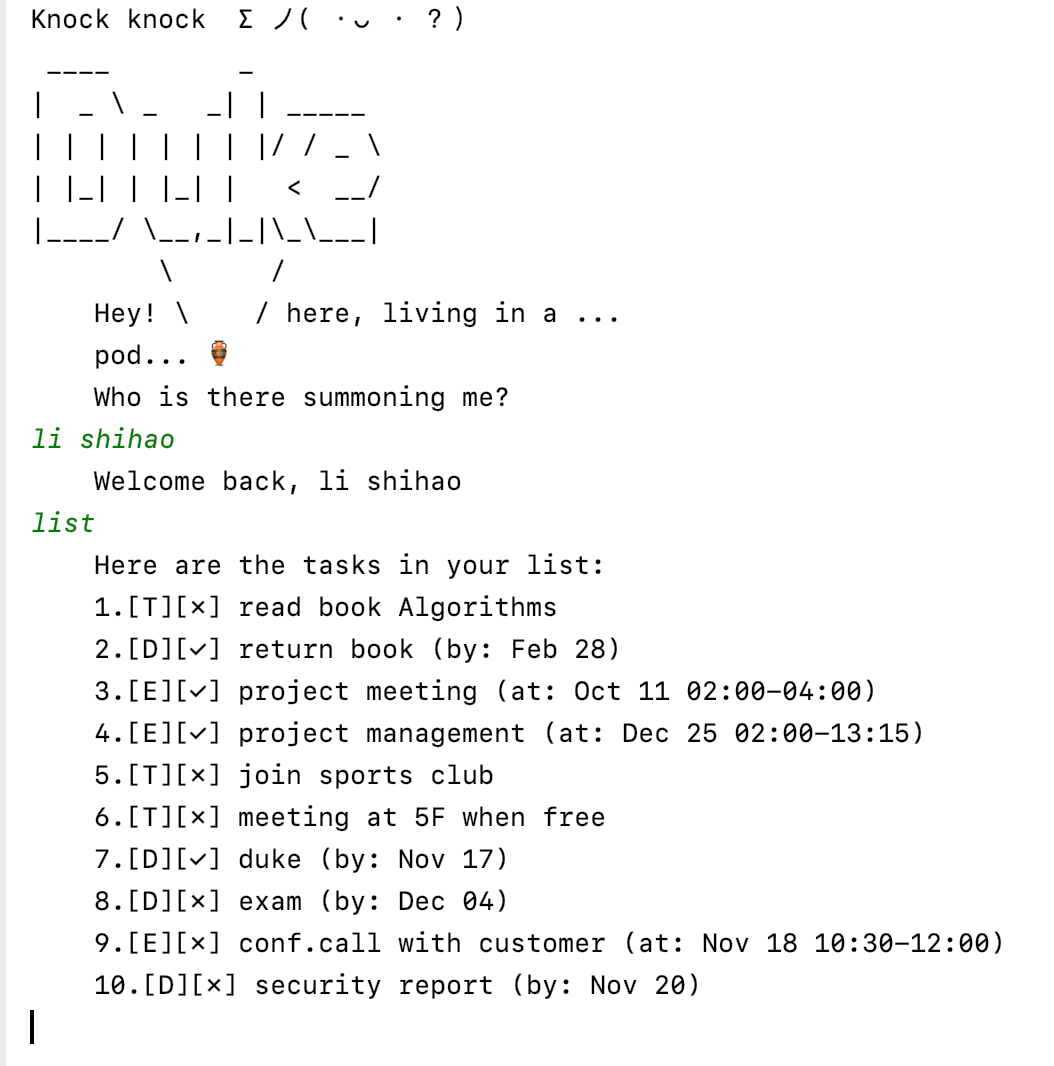
\includegraphics[height= 12.8cm]{list.png}
\caption{Screenshot - \texttt{list}} 
\label{startold}
\end{figure} 


\section* {Level-3 Describe the commands for marking/unmarking tasks as done.} 
\begin{figure}[h]
\left
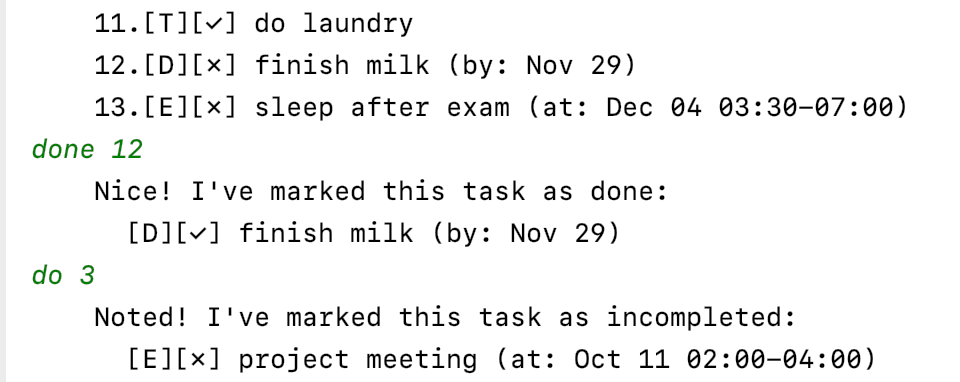
\includegraphics[width = 11.4cm]{done.png}
\caption{Screenshot - \texttt{done, do + task no.}} 
\label{startold}
\end{figure} 

\section* {Level-5 Describe what kind of errors Duke can handle} 
\begin{figure}[h]
\left
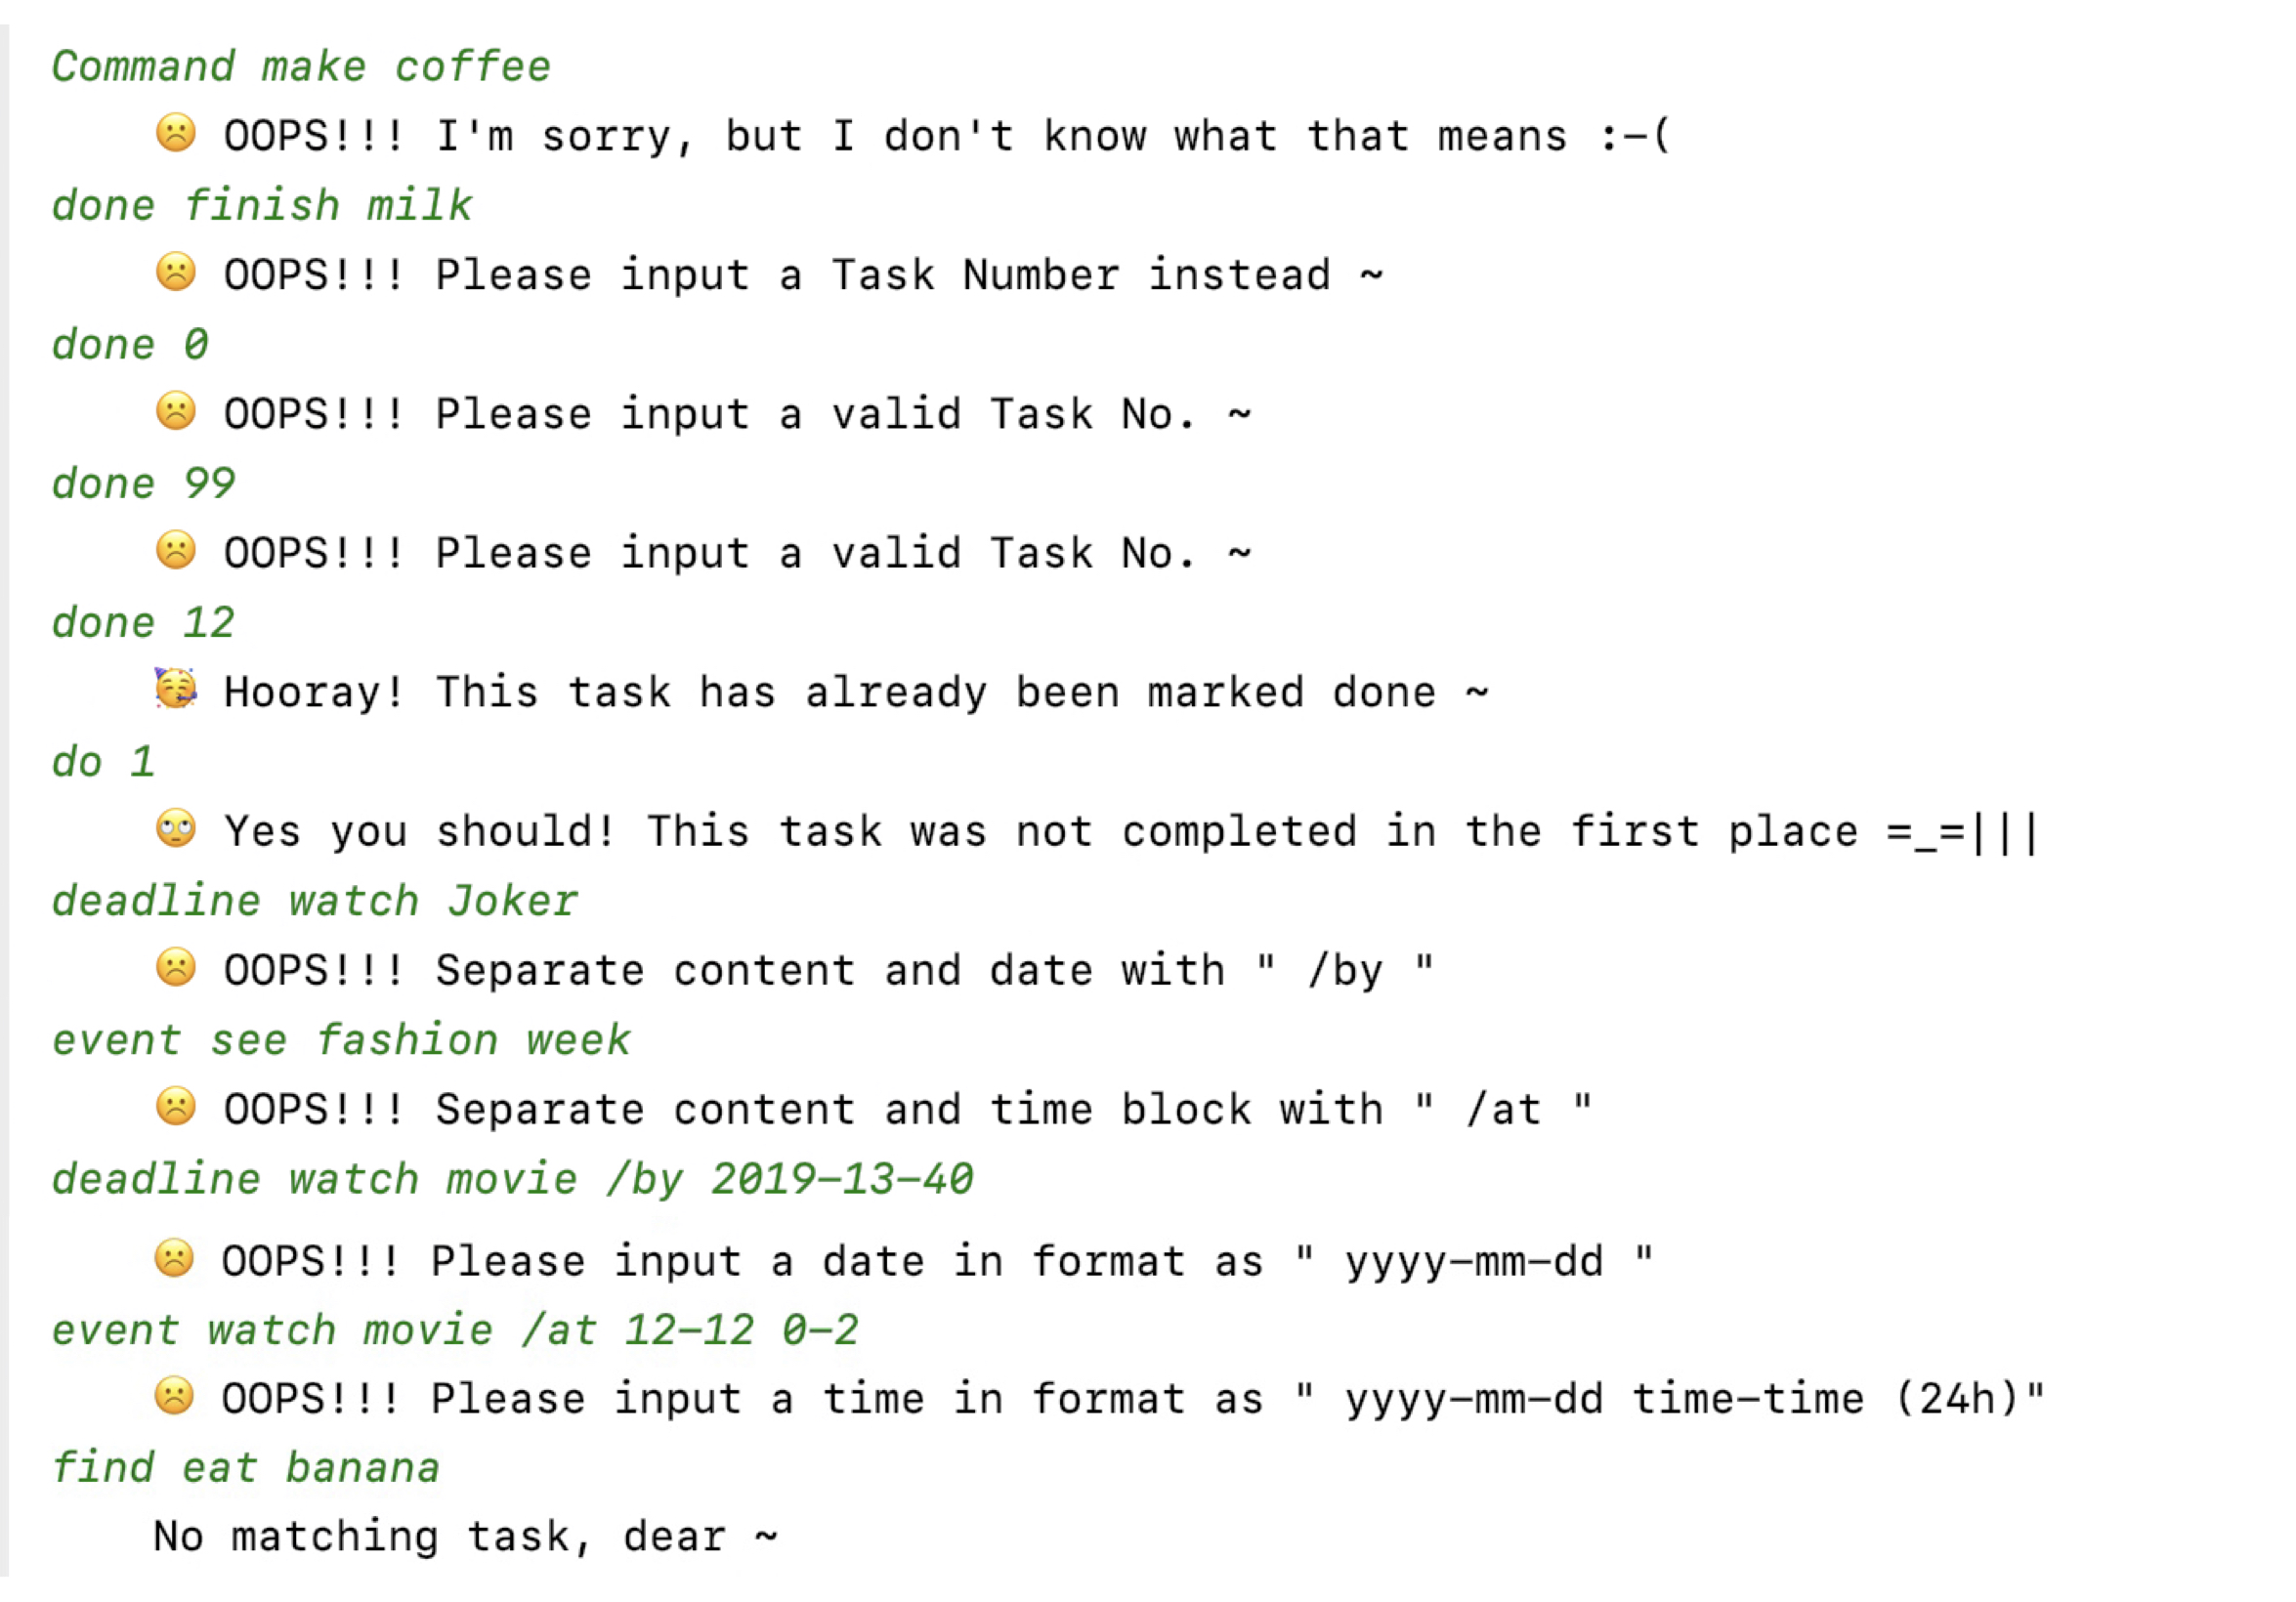
\includegraphics[width = 16cm]{error.png}
\caption{Screenshot - There are also error messages handling file access error} 
\end{figure} 


\section* {Level-6 Describe the commands for deleting tasks} 

\begin{figure}[H]
\left
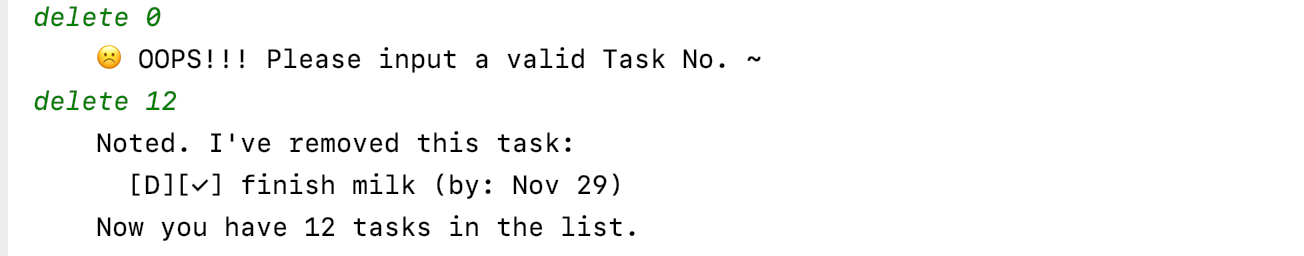
\includegraphics[width = 15.4cm]{delete.png}
\caption{Screenshot - \texttt{delete + task no.}} 
\end{figure} 


\section* {Level-7 Give a sample of the tasks as they are stored in the hard disk} 

\begin{figure}[H]
\centering
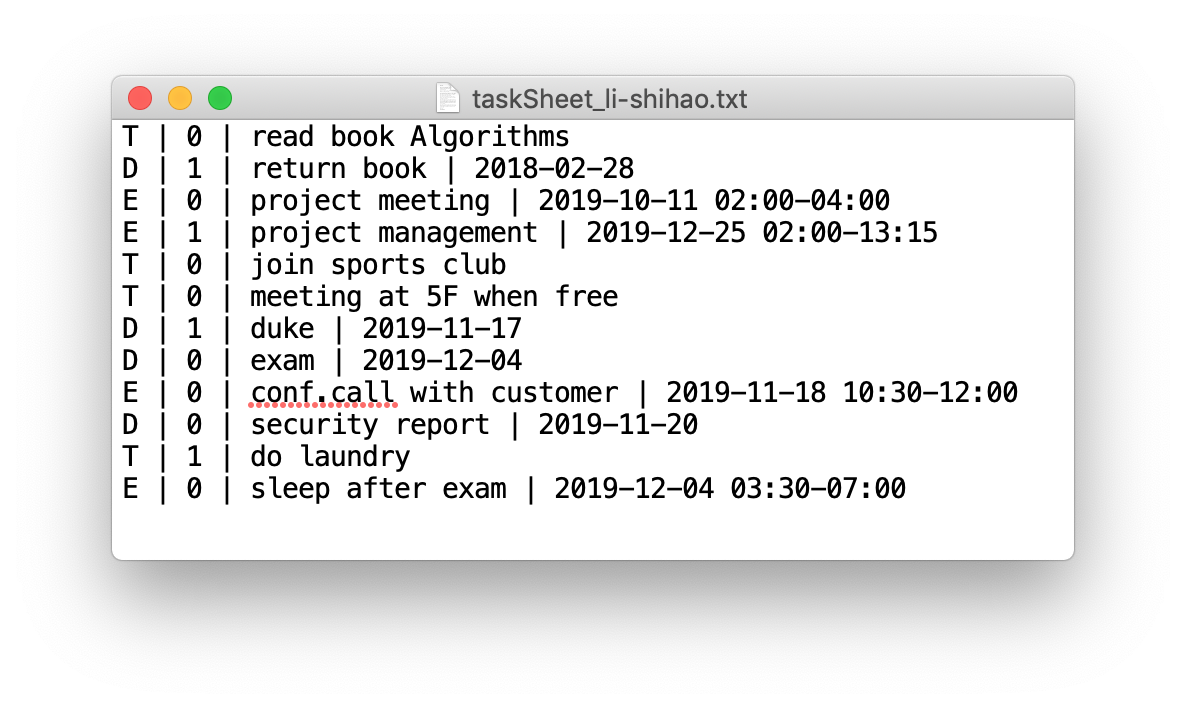
\includegraphics[width = 13.8cm]{file.png}
\caption{Screenshot - File \texttt{taskSheet\_user-name.txt}} 
\end{figure} 

\section* {Level-8 Explain how Duke uses dates/times} 
Date is a property for Deadline type of task, time is property for Event type of task. 
Date can be use to sort tasks of Deadline type in chronological order.  

\section* {Level-9 Describe the commands for searching for tasks.} 
\begin{figure}[H]
\centering
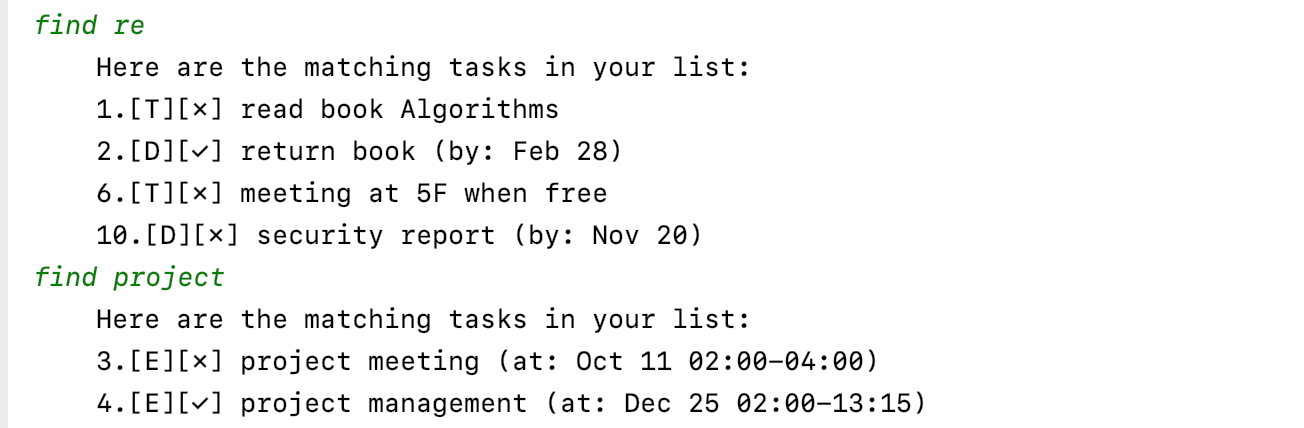
\includegraphics[width = 15.4cm]{find.png}
\caption{Screenshot - Search tasks (notice that the task no. is correct)} 
\end{figure} 


\section* {Level-10 Individual feature: If you implemented an individual feature, describe that feature} 
Sort Deadline tasks in order that oldest date on the top:
\begin{figure}[H]
\centering
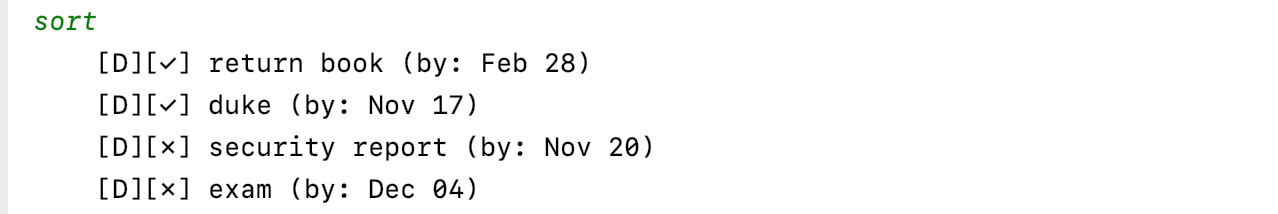
\includegraphics[width = 15.4cm]{sort.png}
\caption{Screenshot - Deadlines \texttt{sort}} 
\end{figure} 

\section* {Other features Describe other features you implement} 
Multiple users can use this program, as long as they remember their usernames, they could get back their tasks. After starting the program, first thing is to enter your username. If you are an existing user, duke will greet you with your username and you can list out all the tasks you had created since last time; If you are a new user, type your desired username, and next time use it to log in to the system.  

\section* {A-MoreOOP Give a class diagram to match your code} 
Refer to Appendix \emph{Figure\ref{class}} \hookleftarrow  click

\section* {A-MoreOOP Give at least one object diagram illustrating the state of your program at some point} 
Refer to Appendix \emph{Figure\ref{object}} \hookleftarrow  

\section* {A-MoreOOP Give at least one sequence diagram illustrating an object interaction in your product} 
Refer to Appendix \emph{Figure\ref{sequence}} \hookleftarrow  

\section* {A-JavaDoc: Give at least 2 javadoc comments from you code} 
\begin{figure}[H]
\centering
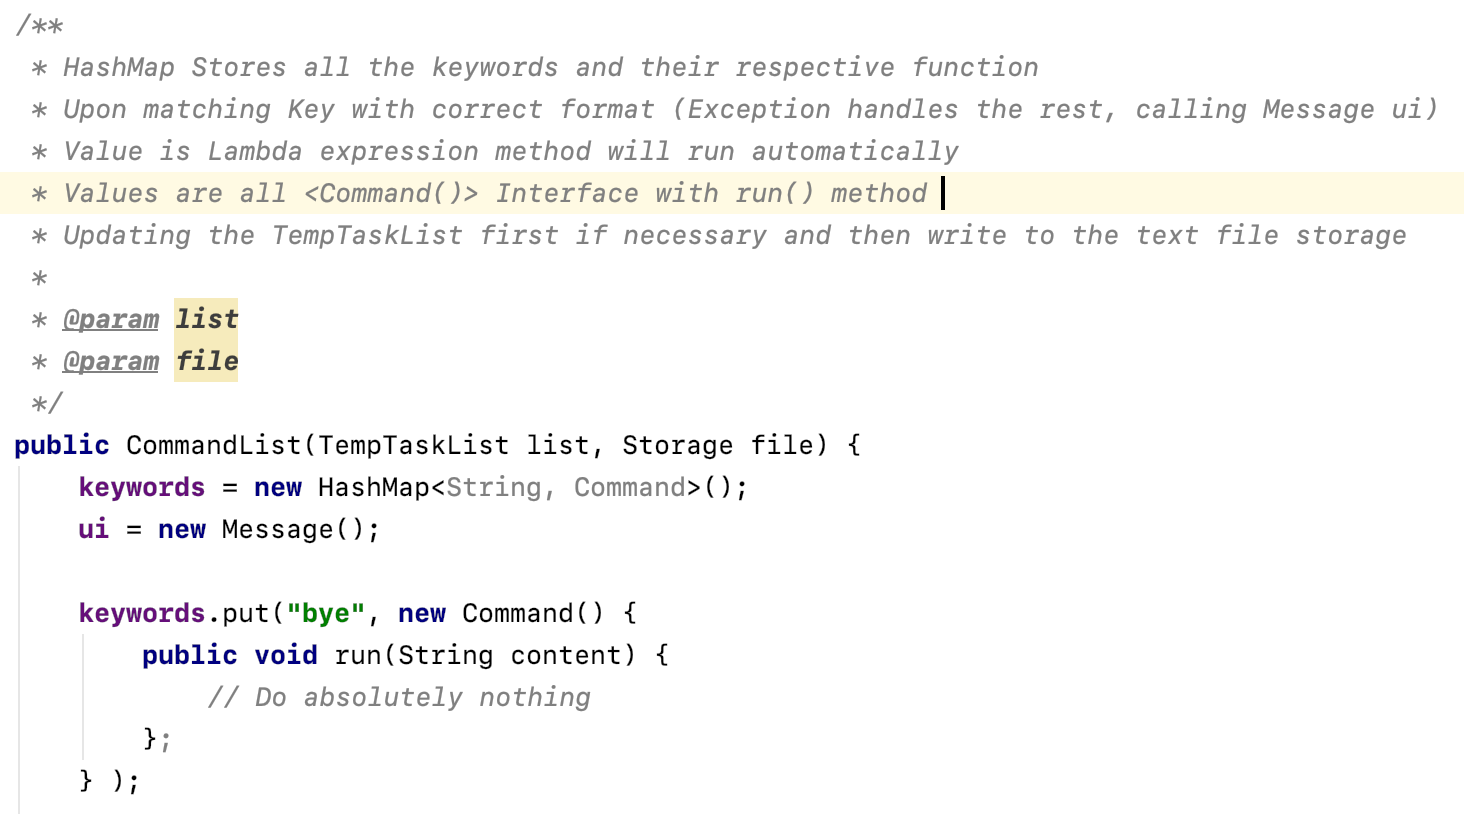
\includegraphics[width = 15.4cm]{jdoc.png}
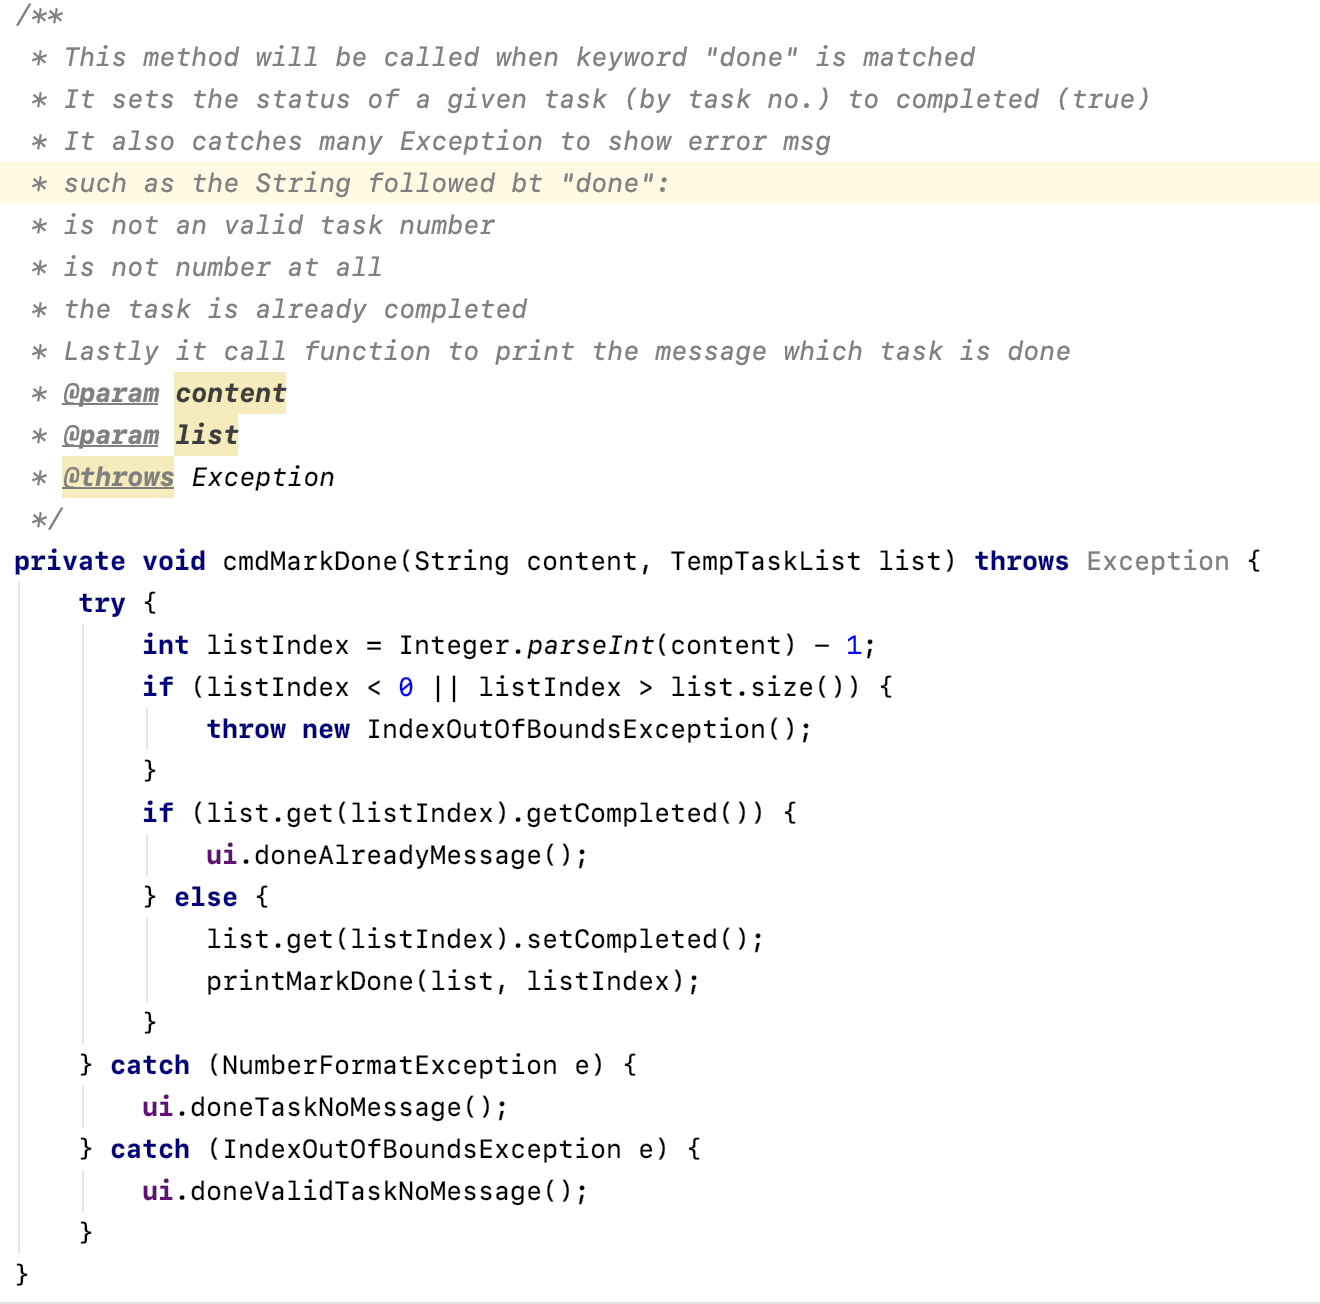
\includegraphics[width = 14.8cm]{jdoc2.png}
\caption{Screenshot - JavaDoc snippets} 
\end{figure} 


\section* {A-JUnit: Give 2-3 JUnit test methods from your code} 
refer to code

\section* {A-Assertions: Give at least 2 code segments that contain assertions you added to your code} 
refer to code 

\section* {Suggested test commands Give a list of commands a tester can execute in sequence to examine your product. Cover all features in a reasonable order: } 
\begin{verbatim}

li shihao
list
hello world
todo read reports 
deadline mark paper /by 2019-12-24
event marathon /at 2019-12-25 10:15-15:30
event firework party /at 2020-01-01 0-4
delete 99
done 0
done 2
do 1
done 1
do 1
sort
find money
find exam
delete 12
list

bye
\end{verbatim}

\clearpage 
\begin{landscape}
\appendixpage


\begin{figure}[h]
\centering
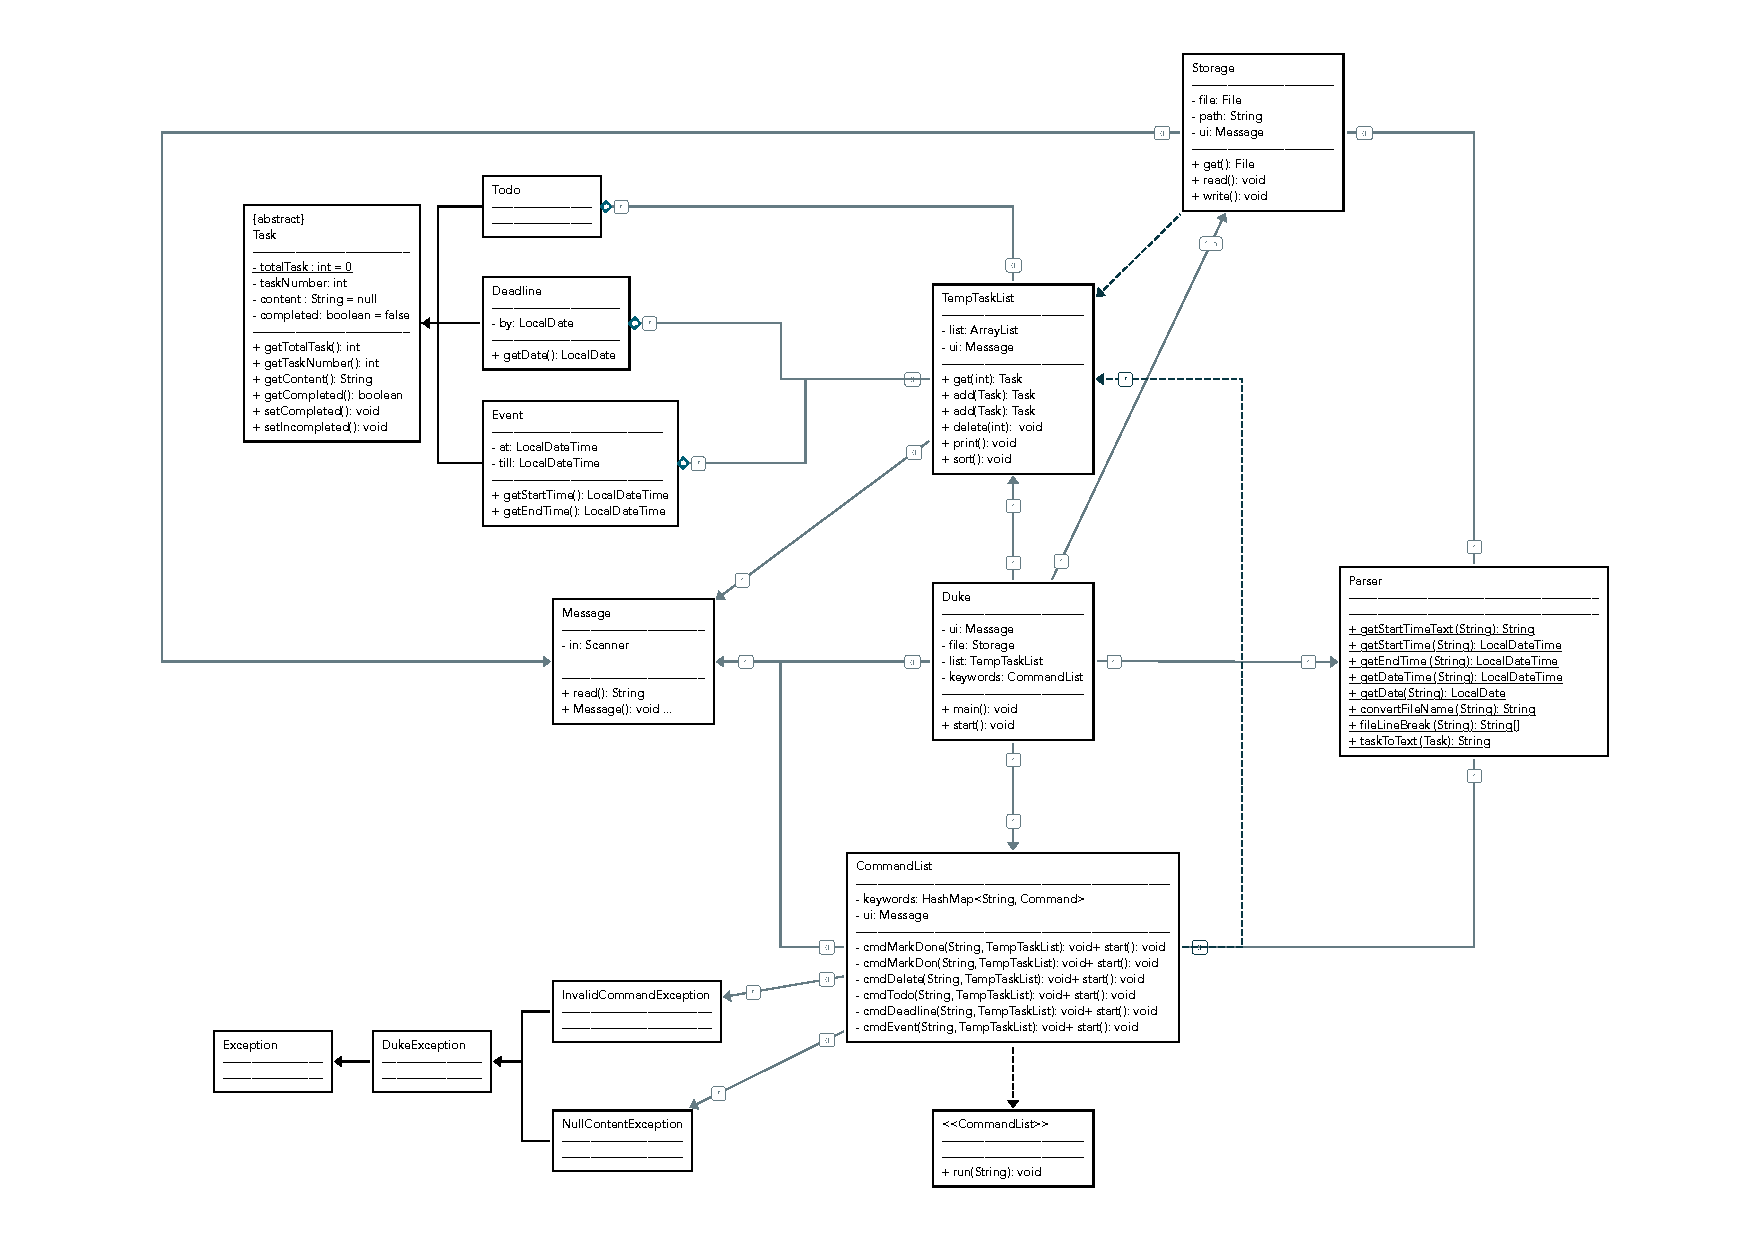
\includegraphics[width = 15.6cm]{class.pdf}
\caption{Screenshot - Class Diagram} 
\label{class}
\end{figure} 
\clearpage

\\When just started the program, a new Duke object will be initiated to call the start() method. 
Duke initiates Message ui, Storage file, TempTaskList list, and pass file and list as parameters to initiate CommandList keywords. 
\begin{figure}[H]
\centering
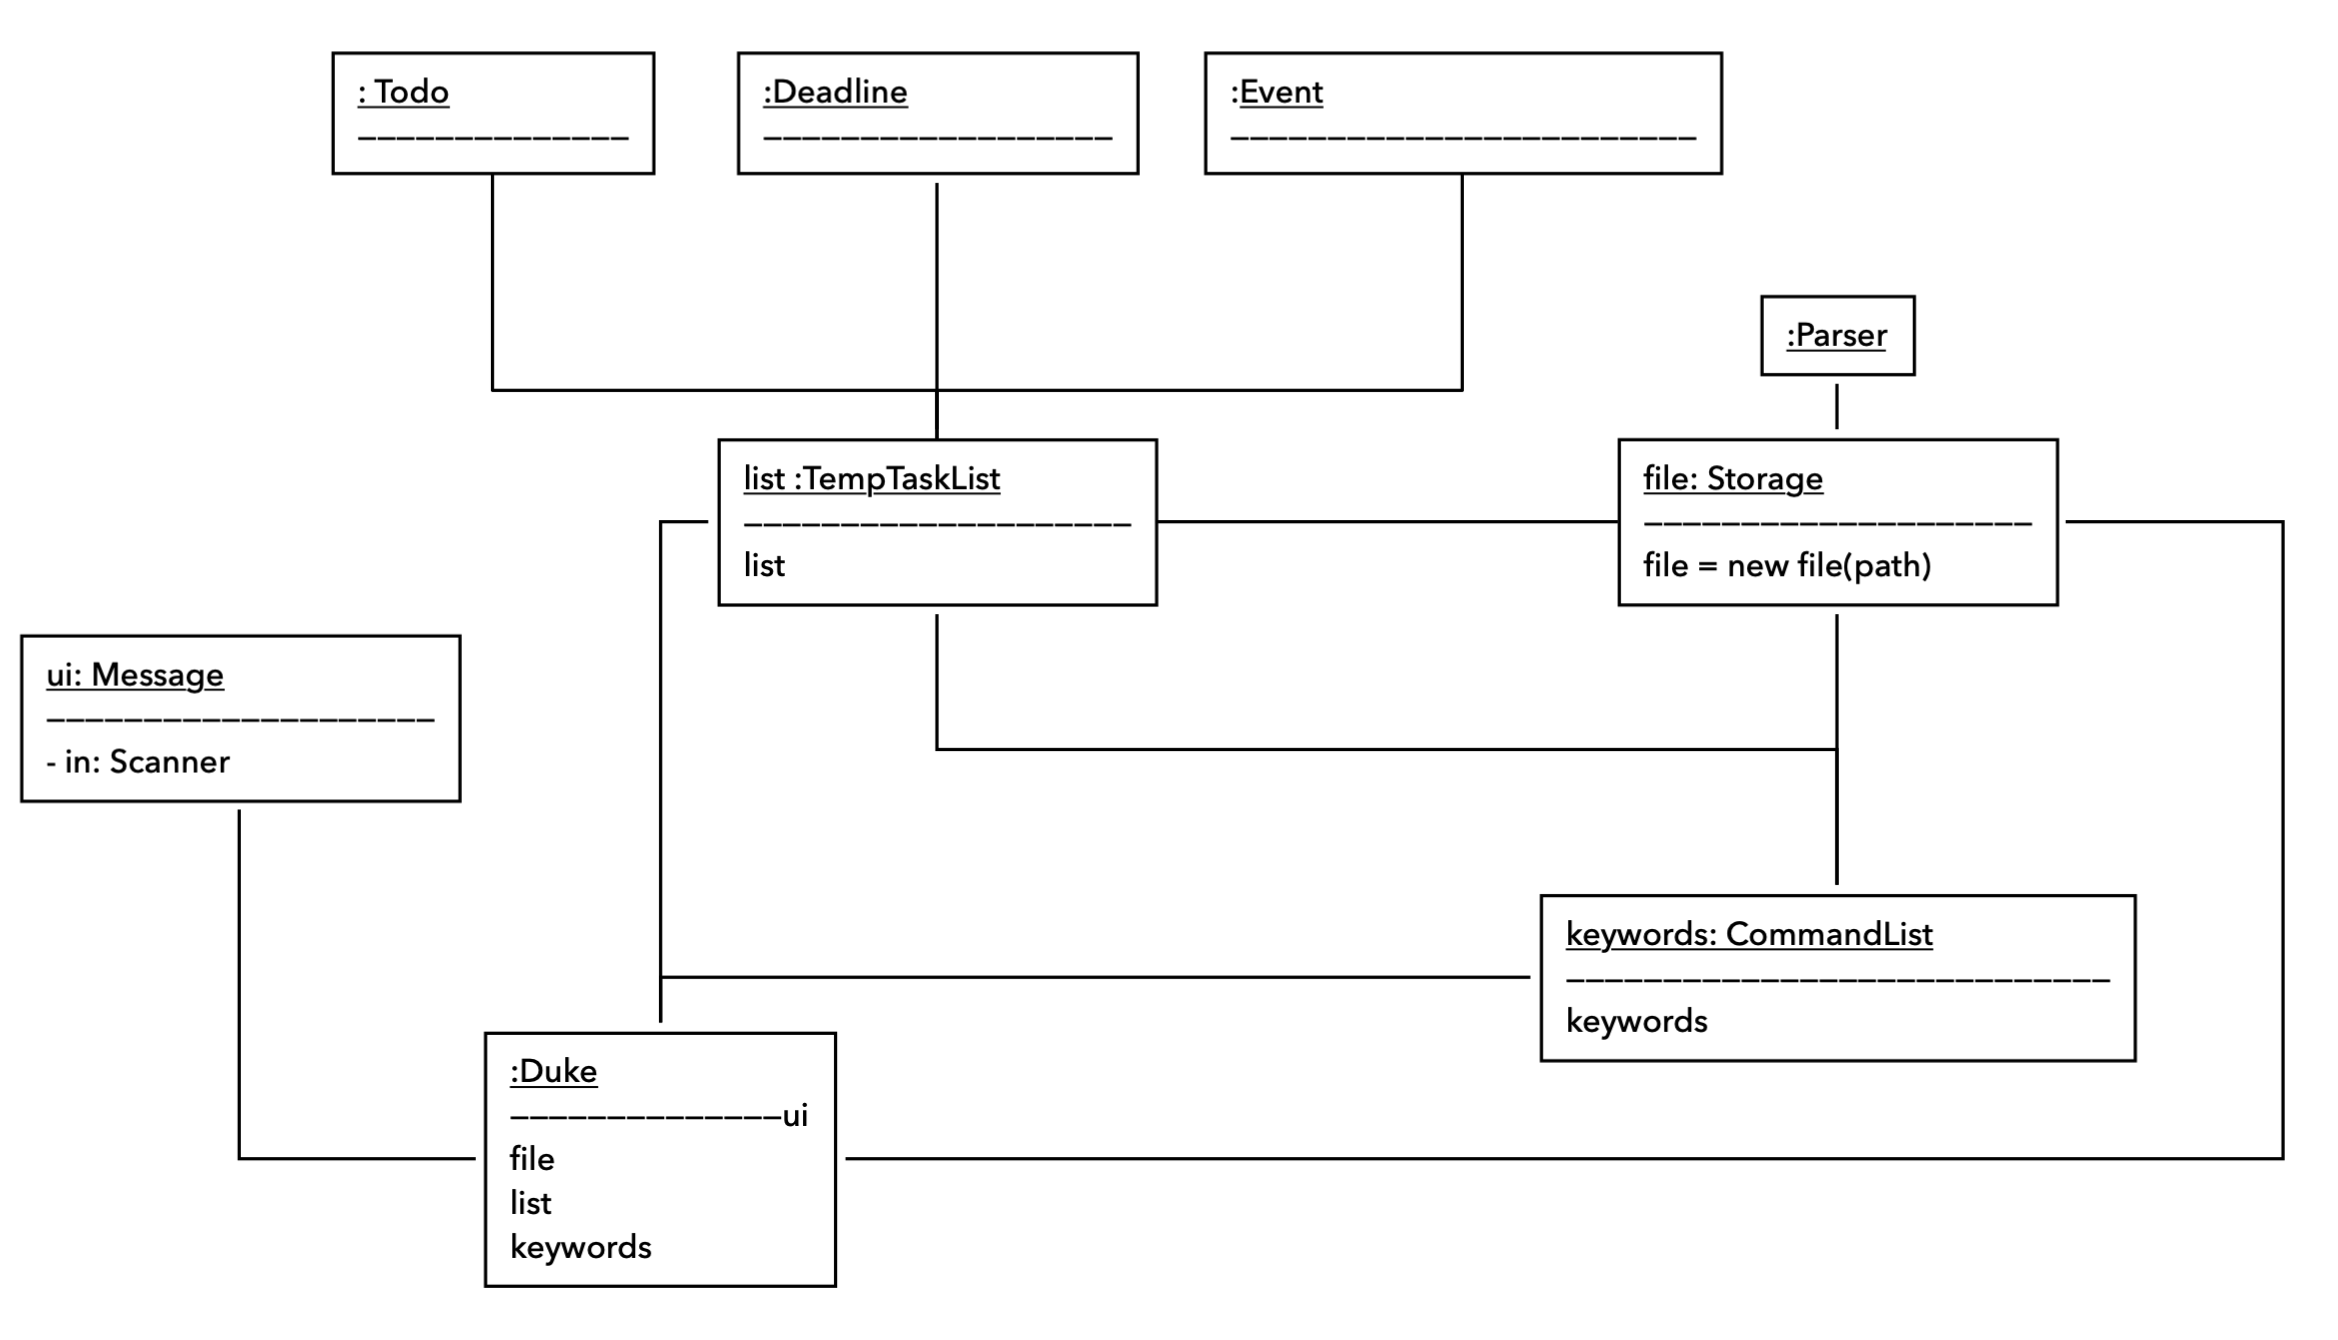
\includegraphics[width = 15.4cm]{object.png}
\caption{Screenshot - Object Diagram} 
\label{object}
\end{figure} 


\begin{figure}[h]
\centering
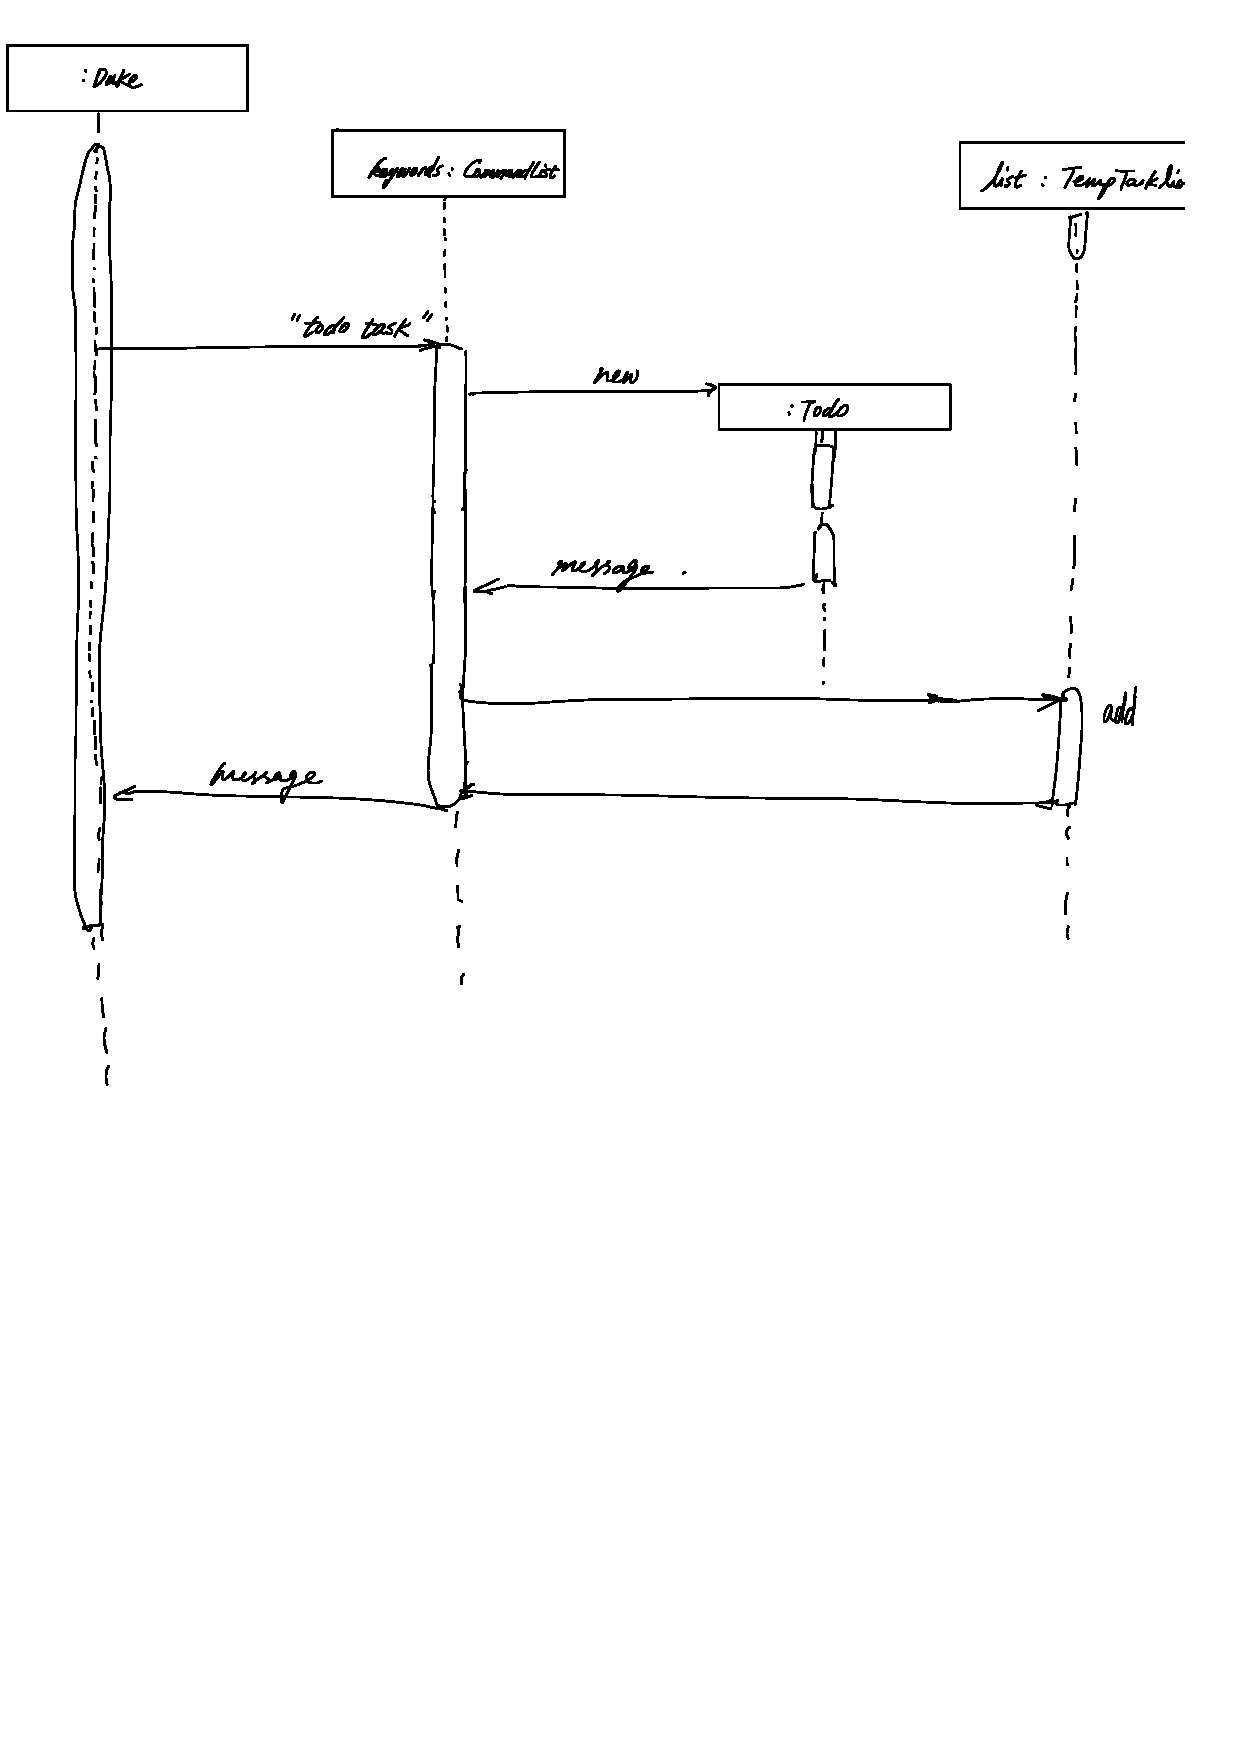
\includegraphics[width = 15.4cm]{sequence.pdf}
\caption{Screenshot - Sequence Diagram} 
\label{sequence}
\end{figure} 

%\printbibliography

%\bibliography{assgn1}


\end{document}













